%\begin{savequote}[75mm] 
%Nulla facilisi. In vel sem. Morbi id urna in diam dignissim feugiat. Proin molestie tortor eu velit. Aliquam erat volutpat. Nullam ultrices, diam tempus vulputate egestas, eros pede varius leo.
%\qauthor{Quoteauthor Lastname} 
%\end{savequote}

\chapter{Identification d'œuvres}
\label{chap:similarite}
%%%%%%%%%%%%%%%%%%%%%%%%%%%%%%%%%%%%%%%%%%%%%%%%%%%%%%%%%
%														%
%		INTRODUCTION									%
%														%
%%%%%%%%%%%%%%%%%%%%%%%%%%%%%%%%%%%%%%%%%%%%%%%%%%%%%%%%%

Comme énoncé précédemment, le système GUIMUTEIC doit être capable de reconnaître l'environnement de l'utilisateur afin de lui donner les informations qu'il désire sur ce qui l'entoure.
Pour identifier cet environnement, nous nous basons sur la reconnaissance d'œuvres, ou instances, et de points d'intérêts. 
Cette reconnaissance d'instances, présentée dans la chapitre~\ref{chap:stateoftheart}, peut être faite par recherche d'images. 
Ce chapitre étudie le problème de reconnaissance d'instances dans les images. 
Notre approche, basée sur l'apprentissage de similarité entre les images, repose sur les réseaux de neurones profonds de type siamois à trois branches.




%%%%%%%%%%%%%%%%%%%%%%%%%%%%%%%%%%%%%%%%%%%%%%%%%%%%%%%%%
%														%
%		SIMILARITE										%
%														%
%%%%%%%%%%%%%%%%%%%%%%%%%%%%%%%%%%%%%%%%%%%%%%%%%%%%%%%%%
\section{Similarité entre les images}
\label{sec:similarite}
Le reconnaissance d'instances consiste à identifier, sur une image donnée, le ou les objets présents. 
Elle se distingue de la classification d'images, dans le sens où on ne s'intéresse pas à une catégorie d'objet, mais à un objet bien identifié. 
Longtemps basé sur les comparaisons d'images à l'aide d'extraction de caractéristiques visuels sur celles-ci, l'utilisation d'apprentissage automatique donne aujourd'hui les meilleurs résultats, comme montré dans le chapitre~\ref{chap:stateoftheart}.

La reconnaissance d'instances peut se faire à l'aide de recherche d'images, où l'on cherche dans une base de données les images les plus ``ressemblantes'', pour déterminer quel objet est visible sur l'image. 
Cette tâche revient donc à déterminer ce qu'est la ressemblance entre deux images. 
Dans notre cas, similarité signifie avoir la même instance. 
Dans le cas idéal, nous souhaiterions avoir la fonction similarité $S$ définie par:

\begin{equation}
S(I_1, I_2) = 
  \begin{cases}
   1       & \quad \text{si } I_1 \text{ et } I_2 \text{ contiennent le même objet}\\
   0  & \quad \text{ sinon }
  \end{cases}
\label{eq:similarite}
\end{equation}

Dans la suite de ce chapitre, le but sera d'approximer cette fonction S.
Une fonction approximée de S tend vers 1 si les images sont similaires.
Pour déterminer l'objet présent dans les images, nous retrouvons les images similaires dans la base de données. 
Comme montré sur le schéma~\ref{fig:rechercheimage}, la recherche d'image permet de classer les images, et ainsi définir la fonction de similarité en fonction de score de ressemblance entre les images.


\begin{figure}%
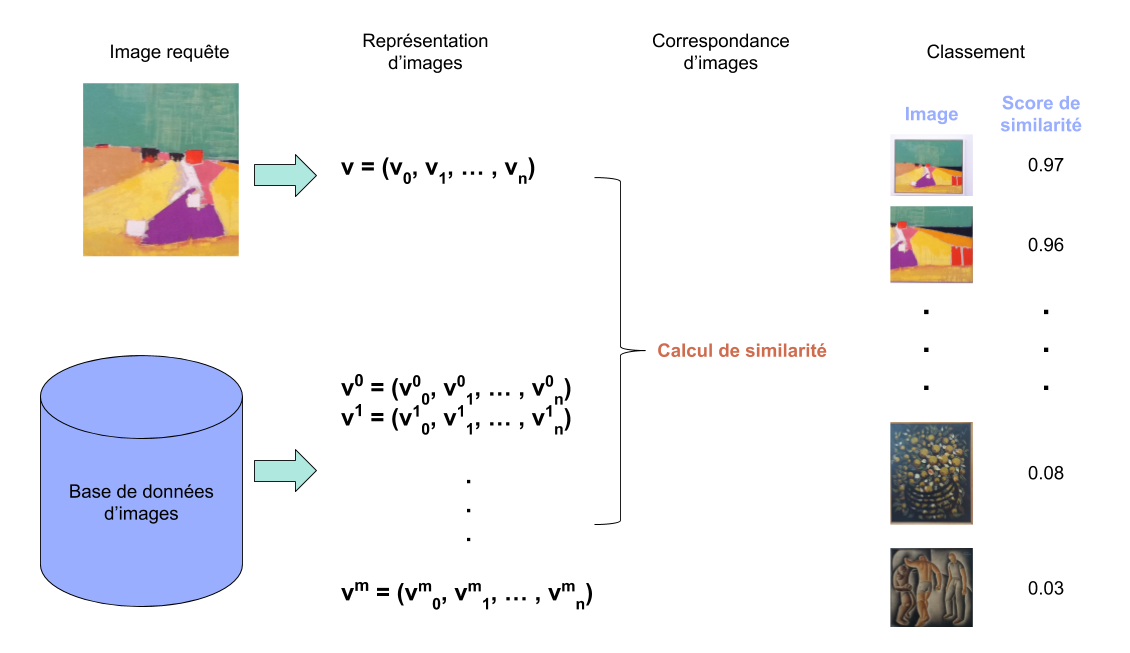
\includegraphics[width=\columnwidth]{figures/rechercheimage.png}%
\caption{Exemple fictif de recherche d'image par le contenu. Le classement représente la similarité entre les images.}%
\label{fig:rechercheimage}%
\end{figure}
 
Nous voyons sur le schéma~\ref{fig:rechercheimage} que pour calculer la similarité des images, nous avons besoin de créer une représentation commune des images $V$. Nous avons exploré dans le chapitre~\ref{chap:stateoftheart} différents moyens de créer ses représentations, à l'aide de descripteurs visuels, ou par apprentissage automatique. En ce basant sur cet état de l'art, il apparait que les méthodes à base de réseaux de neurones profonds, notamment grâce aux réseaux siamois, permettent les meilleurs résulats. 

 
\section{Représentation d'image et similarité}

Pour comparer les images, celles-ci doivent avoir une représentation commune qui permet un calcul de similarité.
Pour créer une représentation commune des images, nous créons un espace de projection de dimension $N$, où chaque images est représentée par un vecteur $V$, son plongement.
La caractéristique principale de cet espace est que les distances entre les vecteurs doivent être inversement proportionnelles à la similarité entre les images. 
La distance entre entre $V_1$ et $V_2$ doit être minimale si l'image $1$ et l'image $2$ représentent le même objet.
Comme montré sur le schéma~\ref{fig:imagespace}, le plongement dans cet espace doit regrouper les images similaires ensemble, et les éloignées des autres. 
Ainsi, en projetant l'image requête dans cette espace, nous pouvons déterminer l'objet présent dans celle-ci, à l’aide de la recherche du plus proche voisin.

\begin{figure}
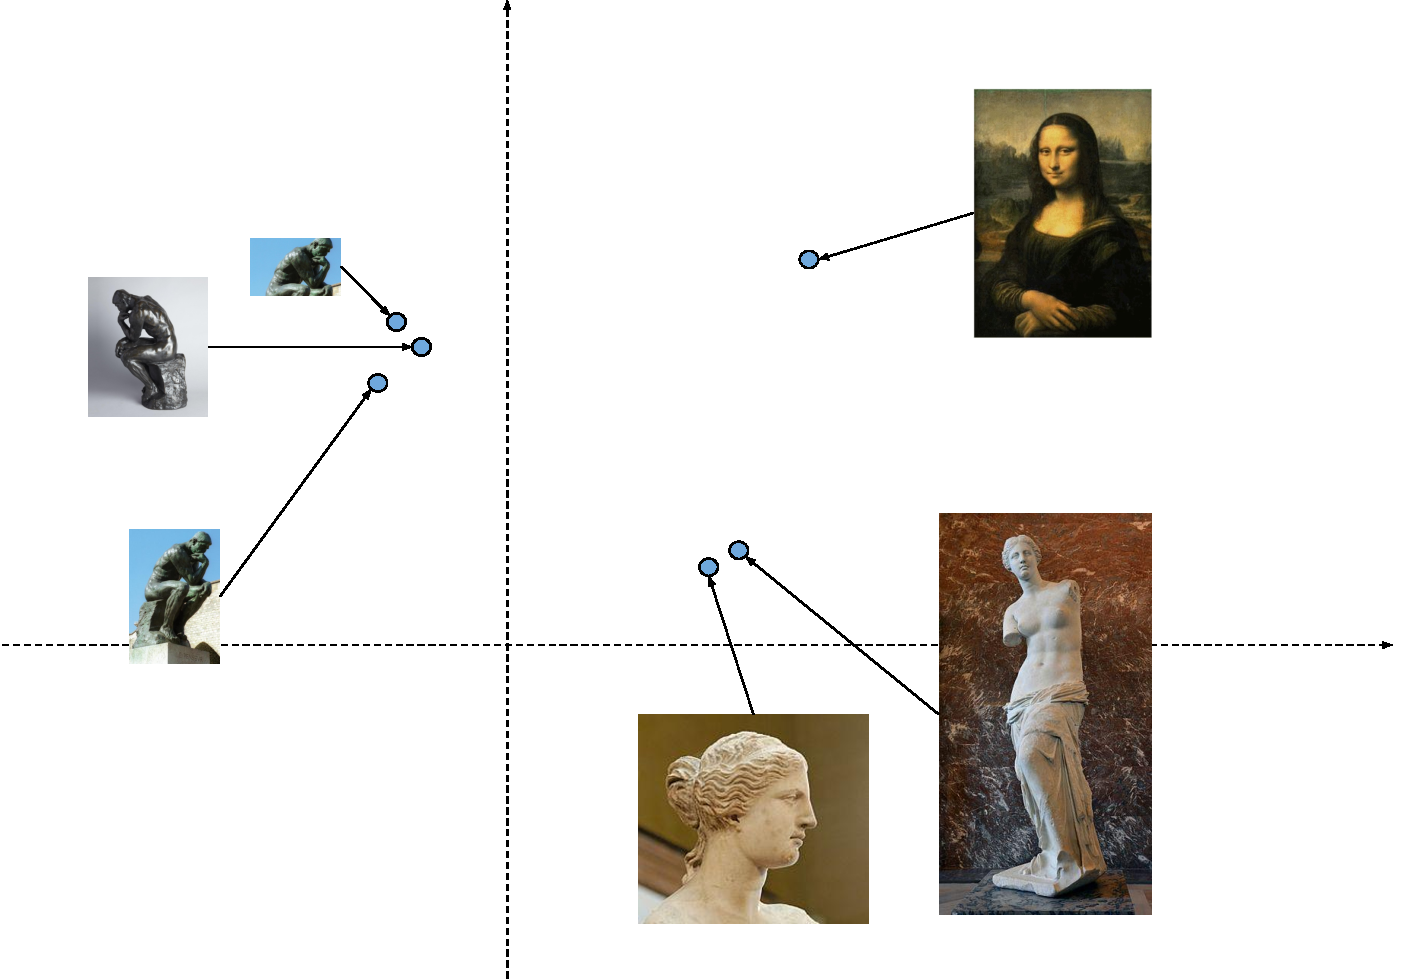
\includegraphics[width=\columnwidth]{figures/imagespace.pdf}
\caption{Projection d’images dans un plan 2D}
\label{fig:imagespace}
\end{figure}


La dimension $N$ de l'espace de projection a une forte importance dans notre contexte. Cette dimension va déterminer une partie du temps de recherche des images. Plus cette dimension est grande, plus les temps de calcul seront important. De la même manière, le type de métriques utilisé pour le calcul de similarité va impacter le coût de calcul. 
L'avantage d'utiliser une méthode d'apprentissage automatique, est que nous pouvons établir la fonction objectif de l'apprentissage en fonction de la métrique qui nous intéresse. 


\section{Plongement des images}

Nous souhaitons apprendre une projection des images, un plongement, qui capture la similarité entre les images. 
Pour le construire, nous utilisons un réseau de neurones, dont la sortie est la projection de dimension $N$. 
Nous avons montré dans le schéma~\ref{fig:extractfeatures} de la section~\ref{sec:extractfeatures} qu'il est possible d'extraire les caractéristiques depuis n'importe quelle couche cachée d'un réseau de neurones pour créer un représentant de l'image. 
Dans notre cas, nous voulons créer un plongement $V \in \mathbb{E}$ qui projette l'image dans un espace euclidien $\mathbb{E}$ de dimension $N$.

Nous créons un réseaux de neurones qui produit le plongement $P$ des images.
Pour l'apprentissage de ce réseau, nous nous basons sur la seule information dont nous disposons, c'est-à-dire un ensemble d'images avec leur étiquette pour savoir si elles représentent le même objet. 
Etant donnée une image $I$ parmi l'ensemble des images disponibles $\tau$, nous définissons l'ensemble des images $\tau_p(I)$ contenant le même objet que l'image $I$ (équation~\ref{eq:pi}), et inversement $\tau_n(I)$ l'ensemble des images ne contenant pas le même objet que $I$ (équation~\ref{eq:ni}).

\begin{equation}
\tau_p(I) = \left\{ x \in \tau | S(I, x) = 1 \right\}
\label{eq:pi}
\end{equation}

\begin{equation}
\tau_n(I) = \left\{ x \in \tau | S(I, x) = 0 \right\}
\label{eq:ni}
\end{equation}



\section{Réseau siamois}

Dans le chapitre~\ref{chap:stateoftheart}, nous avons détaillé l'apprentissage à base de réseaux siamois. 
Ces derniers permettent d'apprendre une similarité entre les images~\cite{schroff2015facenet}. 
Nous nous basons sur les réseaux siamois à trois branches, présentés sur le schéma~\ref{fig:tripletloss}.
Ceux-ci obtiennent les meilleures performances pour la recherche d'instance~\cite{gordo2016deep}, et sont plus adaptés pour les collections de taille réduite.


Là où Schroff et al.~\cite{schroff2015facenet} peuvent se baser sur une grande collection d'image de visage pour apprendre les différences, nous ne disposons pas de corpus aussi important pour la recherche muséale. 
Pour être capable d'utiliser des réseaux profonds de grandes tailles, qui fournissent généralement les meilleures résultats, nous devons utiliser du transfert de connaissances (présenté en section~\ref{sec:transfertlearning}). 
Comme nous allons réaliser une première partie de l'apprentissage sur ImageNet~\cite{deng2009imagenet}, nous basons donc notre architecture sur des réseaux convolutionnels qui sont capables d'obtenir de bonnes performances sur cette collection.
Une fois l'apprentissage réalisé sur ce corpus, nous pouvons spécialiser notre réseaux pour créer le plongements $P$ qui nous intéressent.
Cette phase d'apprentissage se fait à l'aide de triplets d'images.
Ces triplets représentent (équation~\ref{eq:triplets}) une image de \textbf{référence}  $I_r$, une image \textbf{positive}  $I_p$ représentant le même objet que l'image référence, et une image \textbf{négative}  $I_n$ qui contient un objet différent.

\begin{equation}
\Eta = \left\{ (x,y,z) \in \tau^3 | y \in \tau_p(x) \text{ et } z \in \tau_n(x) \right\}
\label{eq:triplets}
\end{equation}

\begin{figure}%
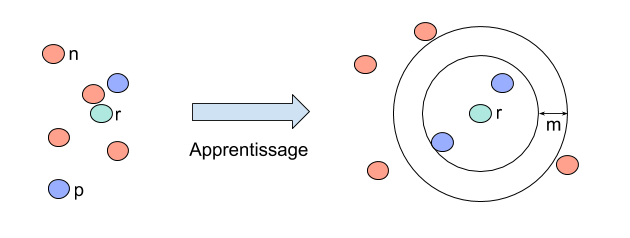
\includegraphics[width=\columnwidth]{figures/Entrainementtriplet.png}%
\caption{Schéma de l'apprentissage du plongement des images, pour une image de références r, avec les images positives p représentant le même objet, et les images n qui contiennent des objets différents.}%
\label{fig:apprentissagetriplet}%
\end{figure}

Le réseau de neurones produit une fonction $P$ de plongement des images dans $\mathbb{E}$. Pour entraîner ce réseau, nous devons définir une \textbf{fonction objectif} associée. 
Cette fonction doit capturer la similarité entre les images.
Nous voulons que $P(I_r)$ soit plus proche du plongement $P(I_p)$ que de $P(I_n)$, comme montré par l'équation~\ref{eq:objectif}, avec $m$ qui représente la marge minimale désirée entre les plongements positifs et négatifs :

\begin{equation}
\forall (x,y,z) \in \Eta, ||x - y|| + m < ||x - z|| 
\label{eq:objectif}
\end{equation}

Cette marge $m$ nous permet de définir un seuil, qui nous permet de déterminer la similarité $S$:

\begin{equation}
S(I_1, I_2) = 
  \begin{cases}
   1       & \quad \text{si } || P(I_1) - P(I_2) || < m\\
   0  & \quad \text{ sinon }
  \end{cases} 
\label{eq:simmargin}
\end{equation}



Nous nous intéressons uniquement à la projection sur l'hypersphère unité des plongements (equation~\ref{eq:hypersphere}). 
Ce qui permet d'utiliser le produit scalaire uniquement pour calculer la similarité cosinus entre les embeddings et mène à un calcul de gradient moins coûteux.
\begin{equation}
\forall I \in \tau, P(I) = \frac{P(I)}{||P(I)||},\text{ donc }||P(I)|| = 1
\label{eq:hypersphere}
\end{equation}
 

Pour l'apprentissage, nous souhaitons donc à minimiser l'équation \textbf{objectif triple}:

\begin{equation}
\mathcal{L}(x,y,z) =  \max(0, P(x) \cdot P(z) - P(x) \cdot P(y) + m)
\label{eq:losstriple}
\end{equation}

pour l'ensemble des triplets $(x,y,z) \in \Eta$. 
Cette fonction de coût est grande si $z$ est similaire à $x$, autrement dit elle est proportionnelle au produit scalaire $P(x)\cdot P(z)$.
Et elle diminue si $y$ est similaire à $x$, c'est-à-dire qu'elle est inversement proportionnelle à $P(x)\cdot P(y)$.
Ce qui correspond sur le schéma~\ref{fig:apprentissagetriplet}, à éloigner les exemples négatifs et rapprocher les exemples positifs pendant l'entrainement.
La fonction $P$ produite par le réseau de neurones doit donc faire tendre la fonction objectif triple vers 0.




\section{Choix des triplets}

Lorsque l'on utilise une fonction objectif triple il faut être particulièrement attentif à la sélection des triplets~\cite{schroff2015facenet}. 
La qualité de l'apprentissage et la vitesse de convergence vont dépendre des triplets présentés au réseau pendant l'apprentissage.
Plus précisément, il existe des exemples plus ou moins ``faciles''.
Il nous faut choisir les triplets pour l'apprentissage pour deux principales raisons : un triplet facile ne fait rien apprendre au réseau et des triplets trop difficiles dès le départ conduisent rapidement à un minimum local ou font s'effondrer le réseau ($P(x) = 0, \forall x$).

Un exemple facile, à gauche sur le schéma~\ref{fig:exemplefacile} correspond à un triplets où les projections sont correctes. Au centre, un exemple difficile correspond au cas où le plongement de l'image négative est plus proche de l'image de référence que celui de l'image positive, et comprend également tous les cas où l’ordre entre positif et négatif n’est pas respecté. Enfin, nous référons à un exemple semi-difficile, à droite, dans le cas où les distances entre les embeddings est correcte, mais l'exemple négatif est dans la marge $m$.


\begin{figure}[htbp]

\begin{subfigure}{0.32\textwidth}
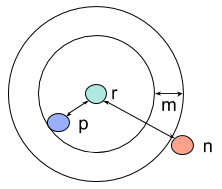
\includegraphics[width=\linewidth]{figures/exemplefaciles.png}
\caption{triplet facile} \label{fig:exemplefacile}
\end{subfigure}
\hspace*{\fill} % separation between the subfigures
\begin{subfigure}{0.32\textwidth}
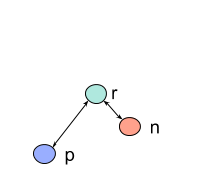
\includegraphics[width=\linewidth]{figures/exempledifficile.png}
\caption{triplet difficile} \label{fig:exempledifficile}
\end{subfigure}
\hspace*{\fill} % separation between the subfigures
\begin{subfigure}{0.32\textwidth}
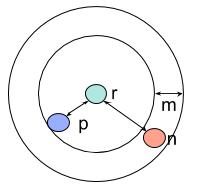
\includegraphics[width=\columnwidth]{figures/exemplesemidifficile.png}
\caption{triplet semi-difficile} \label{fig:exemplesemidifficileb}
\end{subfigure}

\caption{Exemple des différentes configuration des projections possibles. La projection de l'image de référence $r$ est plus ou moins proche des projection de l'image positive $p$ ou de l'image négative $n$.} 
\label{fig:triplets}
\end{figure}




En nous basant sur l'équation~\ref{eq:objectif}, nous pouvons définir un exemple positif facile ou difficile en fonction de la valeur de $||P(x) - P(y)||$ pour un couple d'image $(x,y)$ représentant le même objet. 
Les exemples positifs difficiles $p_d$ sont ceux dont la projection est plus éloignée qu'au moins un des exemples négatifs :

\begin{equation}
p_d(x) = \left\{ y \in \tau_p(x) \middle| \exists z \in \tau_n(x),  \|P(x) - P(y)\| > \|P(x) - P(z)\| \right\}
%p_d = \argmax_{y \in \tau_p(x)} ||P(x) - P(y)||
\label{eq:maxhard}
\end{equation}

Nous définissons de la même manière les exemples négatifs difficiles $n_d$ en fonction de la valeur de $||P(x) - P(z)||$, où les images $x$ et $z$ représentent des objets différents: 

\begin{equation}
n_d(x) = \left\{ z \in \tau_n(x) \middle| \exists y \in \tau_p(x),  \|P(x) - P(y)\| > \|P(x) - P(z)\| \right\}
%n_d = \argmin_{z \in \tau_n(x)} ||P(x) - P(z)||
\label{eq:minhard}
\end{equation}

L'ensemble les \textbf{triplets difficiles} $\Eta_d$ (équation~\ref{eq:hardtriplet}) correspond aux triplets pour lesquels les exemples positifs et négatifs sont diffiles.

\begin{equation}
\Eta_d = \left\{ (x,y,z) \in \Eta \middle| y \in p_d(x) \text{ et } z \in n_d(x) \right\}
\label{eq:hardtriplet}
\end{equation}

Une première stratégie pour la selection des triplets, proposée par Schroff et al.~\cite{schroff2015facenet}, consiste à prendre les triplets semi-difficles, en choisissant les positifs les plus difficiles, et de prendre les exemple négatifs qui sont dans la marges $m$.
Une autre méthode par Gordo et al.~\cite{gordo2016deep}, propose de choisir les $i$ exemples positifs les plus faciles et les $j$ négatifs les plus difficiles, de choisir parmis toutes les combinaisons possibles de triplets celui qui maximise la fonction objectif triple. 
Ce choix semble très pertinent, car il permet de déterminer les exemples qui feront converger le plus rapidement, tout en élimant les images positifs difficiles, c'est-à-dire celles qui représentent la même instance, mais avec trop de différences visuelles. 
Cette méthode demande cependant de parcourir l'ensemble des données d'apprentissage pour calculer la fonction de coût.
Comme le réseau est mis à jour à chaque rétro-propagation, il faut recalculer la fonction de coût assez fréquemment.

Avec nos contraintes spécifiques, à savoir surtout que nous ne disposons que d'un ensemble limité d'exemples positifs, nous choisissons une méthode de selection des triplets hybride entre les deux présentée précédemment. 
Nous choississons l'ensemble des triplets $\Eta_{sd}$, où pour l'ensemble des couples positifs possibles, nous choississons les exemples négatifs semi-difficiles :
\begin{equation}
\Eta_{sd} = \left\{ (x,y,z) \in \Eta \middle| \|P(x) - P(y)\| < \|P(x) - P(z)\| < \|P(x) - P(y)\| + m \right\}
\label{eq:semihardtriplets}
\end{equation}

La figure~\ref{fig:pipelinesimilarite} montre les étapes de l'apprentissage du réseau.
Dans un premier temps, le réseau est appris sur une base de données de grande taille, par exemple ImageNet.
La deuxième étape correspond en un fine-tuning sur la collection du musée.
Ceci permet de spécifier le réseau aux images de musée, étant donné la différence entre les deux collection, ce qui rend la convergence à l'étape suivante plus rapide.
Finalement, nous apprenons le réseau à l'aide des triplets d'image du musée.


Dans un second temps, une fois qu'il n'y a plus de convergence, nous choisissons tous les triplets de $\Eta_d$.

\begin{figure}[htbp]
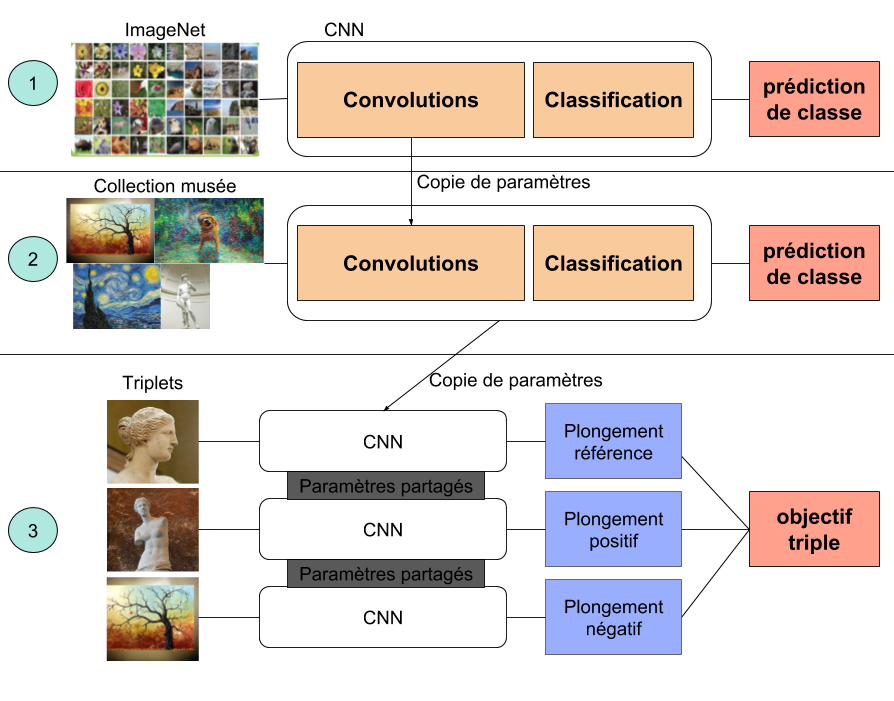
\includegraphics[width=\columnwidth]{figures/pipeline1.png}%
\caption{Pipeline d'apprentissage. L'étape 1 correspond à l'apprentissage du réseau sur une grande collection d'image, ici ImageNet. L'étape 2 est le fine-tuning sur la collection du musée. La troisième étape consiste à apprendre à l'aide du réseau siamois triple.}%
\label{fig:pipelinesimilarite}%
\end{figure}



\section{Évaluation}

Pour évaluer notre première proposition, nous utilisons la collection CLICIDE (détaillée dans la section~\ref{sec:garofou}). 
Ce corpus représente un ensemble de photos d'un musée d'art, et donc surtout des tableaux et peintures, avec différents points de vue sur les oeuvres, et correspond aux contraintes lié à notre projet. La collection GaRoFou (section~\ref{sec:garofou}) vient du musée d'archéologie de Lyon Fourvière, et présente des objets de différentes natures, comme des sculptures, des artéfacts ou des stèles.

Nous comparons notre approche à celles de l'état de l'art, et à diverses méthodes de deep learning. 
Les méthodes à base de descripteurs visuels sur ce dataset ont été explorées précédemment~\cite{portaz2017construction}, avec l’utilisation de SIFT et de sacs de mots visuels. 
Pour identifier l'image similaire dans la base d'image qui va nous permettre de déterminer l'objet présent dans l'image, on recherche l'image la plus proche, ce qui correspond au TOP@1 de la recherche d'image :
 
\begin{equation}
TOP@1(I) = \argmin_{x \in \tau} ||P(I) - P(x)||
\label{eq:simrank}
\end{equation}


\subsection{Autres approches comparées}
Toutes les méthodes comparées utilisent le même type d'architectures, à savoir AlexNet et Resnet, présentés plus en détail dans le chapitre~\ref{chap:stateoftheart}. 
Nous nous comparons principalement aux réseaux siamois à trois branches proposés par Gordo et al.~\cite{gordo2016deep}, avec multi-resolution(Gordo multi-res) et sans (Gordo). 
Pour avoir une idée des autres techniques utilisables, nous montrons les résultats obtenus avec:

\begin{itemize}
  \item Extraction de caractéristiques: Alexnet E et Resnet E (pour Extraction). Un réseau de neurones de type Alexnet ou Resnet est appris sur une grande collection, ici Imagenet. 
	Les images du musée sont ensuite représentées par la sortie d'une des couches du réseau. 
	Nous selectionnons ici la couche caché qui donne les meilleurs résultat dans notre cas, à savoir la couche \textit{fc6} pour Alexnet et \textit{pool5} pour Resnet. 
	\item Fine-tuning et classification des oeuvres: Alexnet Classif et Resnet Classif. Un réseau est appris de manière conventionnelle sur ImageNet, et ensuite un apprentissage fin est réalisé où chaque oeuvre est une classe. Les résultats sont ceux de la classification de chaque oeuvres du corpus de test.
	\item Réseau siamois à double branche: Alexnet SS et Resnet SS (pour Siamois Simple). Un réseau siamois à deux branches est utilisé pour l'apprentissage. La selection des couples se fait de la manière suivante : tous les couples positifs possibles, et le même nombre de couple négatifs, qui correspondent aux exemples les plus difficiles. 
\end{itemize}



\subsection{Paramètres d'apprentissages}

Le fine-tuning sur les deux réseaux utilisés se fait en commençant par la dernière couche entièrement connectée.
Nous apprenons tout d'abord la dernière couche seule, et après stabilisation de la fonction de coût, nous ajoutons à l'entraînement la couche précédente.
Nous continuons ainsi jusqu'à avoir entraîné toutes les couches.
Il est important de ne pas entraîner tous les réseaux d'un seul coup, car lorsque l'on fait un \textit{fine-tuning}, on supprime la dernière couche de classification pour la remplacer par une qui a le bon nombre de sorties.
Cette nouvelle couche étant initialisé aléatoirement, l'erreur de classification sera grande, et propager cette erreur risque de détruire l'ensemble du réseau.
Il est donc nécessaire de procéder couche par couche, car les premières couches sont moins susceptible de devoir être changée, étant donné qu'elles capturent des caractéristiques de plus bas niveau, plus proche de l'image.
De plus, entraîner tout le réseau sur une petite collection entraine un sur-apprentissage, les premières couches ne devraient donc pas être modifiée.

Ces considérations mènent à l'apprentissage suivant:

\begin{itemize}
	\item Pour AlexNet : apprentissage depuis la dernière couche jusqu'à la dernière couche convolutionnelle. Les premières couches convolutifs ne sont pas modifiées.
	\item Pour ResNet : apprentissage de deux dernier bloc de convolution. Contrairement à AlexNet, ResNet repose sur moins de couches entièrement connectées, nous devons donc entraîner davantage de couches convolutionnelles. Comme cette architecture est basé sur des blocs de convolution, nous nous référons à un bloc en entier.
\end{itemize}


\subsection{Etude de l'importance de l'augmentation de données d'apprentissage}
\label{subsec:dataaug}

Toutes les approches présentées se basent sur un fine-tuning.
L'apprentissage sur le corpus de départ, ainsi que sur notre collection, est fait avec une partie d'augmentation de données.
Cette augmentation consiste en différentes perturbations faites sur les images pour éviter un sur-apprentissage du réseau.
Autrement dit, si notre réseau sur-apprend, il aura une capacité limitée à s'adapter à des données différentes de celle d'apprentissage.
Comme nous nous basons sur du transfert de connaissance pour être capable de travailler sur nos collections de petites tailles, cette généralisation est un élément important de notre pipeline.

L'augmentation de données a deux objectifs.
Le premier est d'augmenter le nombre de données présentées au réseau de neurones.
La performance des réseaux de neurones est très fortement liée à la quantité de données sur laquelle on travaille.
Particulièrement dans notre cas, cette augmentation nous permet d'éviter un sur-apprentissage très prononcés sur les petites collections.
Le deuxième objectif est de pallier au manque de variation dans les images de la base d'entrainement. 
En simulant des déplacement de caméra, d'effet de zone, de rotation, on aide le réseau à être invariant à ces transformations.
Trois différentes transformations d'images sont aléatoirement appliquées pendant l'entrainement:


\begin{itemize}
	\item Rotation des images avec une probabilité équivalente pour tous les angles $\{-180, -90, 0, 90, 180\}$.
	\item Changement d'échelle des images avec un facteur aléatoire pour chaque dimension dans l'interval [0.75, 1.25].
	\item Renversement d'image horizontal avec probabilité de $0.5$
\end{itemize}

Le tableau~\ref{tab:dataaugmentation} présente l'influence de chacune des ces perturbations, avec le réseau ResNet-152.
\begin{table*}
\centering
\begin{tabular}{||c|c|c||c|c||}
\hline 
 \emph{Rotation} & \emph{Scaling} & \emph{Flipping} &
 \multicolumn{2}{c||}{\emph{Mean Precision@1 (in \%)}}\\
\hline 
 \multicolumn{3}{||c||}{} & \emph{CLICIDE} & \emph{GaRoFou}\\
\hline  & & & 72.12 & 92.93\\
\hline  \checkmark  & & & 74.55 & 94.02\\
\hline  & \checkmark & & 76.36 & 93.48\\
\hline  & & \checkmark & 72.12 & 94.57\\
\hline  \checkmark & \checkmark & & 76.97 & 94.57\\
\hline  \checkmark & & \checkmark & 75.75 & 94.57\\
\hline  & \checkmark & \checkmark & 78.18 & 93.48\\
\hline  \checkmark & \checkmark & \checkmark & \textbf{79.39} & \textbf{94.57}\\
\hline
\end{tabular}
\caption{Influence de la rotation, de la mise à l'échelle et du renversement sur les résultats avec l'architecture ResNet-152.
\label{tab:dataaugmentation}}
\end{table*}

Le renversement d'image est particulièrement intéressant dans notre cas. 
Il est souvent utilisé dans l'apprentissage de classe, où l'invariance à l'orientation semble important, dans le cas de reconnaissance d'instance cela semble contre-intuitif.
Notamment dans le cadre de collection de tableaux ou de peintures, nous ne voulons pas confondre deux objets qui pourraient être l'image inversée l'un de l'autre. 
Par exemple, l'oeuvre ``4900 Farben'' (``4900 Colors'')\footnote{https://www.gerhard-richter.com/en/art/microsites/4900-colours} de Gerhard Richter est constituée d'un ensemble de panneaux de carrés de couleurs.
Dans ce cas, le renversement d'une image n'est pas équivalente à l'image d'origine, et ne devrait pas être considéré dans l'apprentissage.

Le tableau~\ref{tab:dataaugmentation} montre que la rotation seule ou la mise à l'échelle seule améliorent les résultats. 
Cependant, comme attendu, le renversement seul n'améliore pas l'apprentissage.
Mais n'importe quelle combinaison de perturbation donne de meilleurs résultat que toute les transformations seules, et ce même en considérant le renversement.
De ces résultats nous pouvons conclure que n'importe quelle augmentation de données à travers des perturbations est toujours utile, même pour la reconnaissance de peinture dans le cadre de la collection CLICIDE.
Pour la collection GaRoFou, n'importe quelle perturbation aide l'apprentissage, mais la combinaison de différente transformations ne change pas les résultats.
Cela peut être dû à la plus grande diversité des objets présents dans la collection, ainsi qu'à leur caractère tri-dimensionnel.


\subsection{Résultats}
\label{sec:resultatsimilarite}

\begin{table*}
\centering
\begin{tabular}{|l|c|}
\hline & {\emph{TOP@1 (in \%)}}\\
\hline & \emph{CLICIDE}\\
\hline \emph{Descripteurs Visuels~\cite{portaz2017construction}} & 70.08\\
\hline \emph{Gordo~\cite{gordo2016deep}} & 90.3 \\
\hline \emph{Gordo multi-res~\cite{gordo2016deep}} & \textbf{92.73} \\
\hline \emph{AlexNet E} & 72.73 \\
\hline \emph{AlexNet Classif} & 78.18 \\
\hline \emph{AlexNet SS} & 75.76 \\
\hline \emph{ResNet E} & 72.12 \\
\hline \emph{ResNet Classif} & 79.39 \\
\hline \emph{ResNet SS} & 85.45 \\
\hline \emph{Architecture AlexNet} & 79.39\\
\hline \emph{Architecture ResNet} & \textbf{92.73}\\
\hline
\end{tabular}
\caption{Évaluation des différentes méthodes d’apprentissage pour la projection des images sur le collection CLICIDE.
\label{tab:resultatssansregion}}
\end{table*}

Tout d'abord, nous pouvons voir sur le tableau~\ref{tab:resultatssansregion} que les méthodes à base de descripteurs visuels ingéniérés sont dépassés par toutes les méthodes à base de réseaux de neurones, même si nous travaillons sur une collection d'image de taille réduite. Pour toutes les méthodes proposés, exception faite de l'extraction de caractéristique, une architecture de type Resnet obtient de meilleurs résultats. Pour l'extraction de caractéristiques depuis un réseau pré-entraîné, il en va de la nature de ces réseaux qui explique que Alexnet ait de meilleures performances. Là où Alexnet est une suite de convolution et de maxpooling, Resnet est une série de bloc avec des skip-connection. Que l'extraction sur une couche donnée donne de moins bons résultats signifie juste que dans ce cas les réseaux de retiennent pas l'information de la même manière. Il est intéressant de noter que malgré la petite taille de la collection et d'un grand manque de diversité dans les images (toutes avec le même fond, dans le même musée, etc), le fine-tuning reste intéressant pour améliorer les résultats.

Nous remarquons surtout que les meilleurs résultats sont obtenu avec notre approche, mais également avec l'approche de Gordo. Bien que ces résultats soient surprenamment haut pour cette approche, car les embeddings ne sont pas appris pour cette collection en particulier, plusieurs arguments peuvent expliquer les de si bon résultats. 
Tout d'abord, le réseau proposer par Gordo est appris sur la collection ..., qui dispose d'un grand nombre d'exemples et d'une grande variabilité, qui se prête donc bien à la généralisation sur un autre corpus. 
Dans cette collection, une forte disparité entre les objets existe, ainsi que de très grand écart de point de vue et de distance de zoom. 
Il n'est donc pas étonnant que les plongements créés soient capables d'exprimer de manière convaincante la similarité entre les images. 
De plus, ce réseau dispose d'une partie de proposition de région d'intérêts. 
Dans le cadre de la recherche d'instance dans les images, la détection de la position de l'objet dans l'image est un élément clef, que nous n'avons pas pour le moment pris en compte dans notre approche. 
Lors de la création de l'embedding de l'image, nous voulons que celui ci représente l'objet présent dans l'image au mieux, en faisant fi du fond, d'autres objets moins visibles, ou du bruit. 

Nous avons proposé une nouvelle fonction objectif, basé sur le produit scalaire, ainsi qu'une nouvelle sélection de triplets, le tout dans un nouveau pipeline d'apprentissage adapté à notre problème, et à nos collections.
Notre proposition obtient des résultats proches de ceux de l'état de l'art, avec un réseau plus simple, sans proposition de région, dû aux limitations d’annotation des collections.
Avoir un réseau capable de détecter les régions d'intérêt, et de créer une représentation uniquement de la région où se situe l'objet semble être un éléments clé pour produire un plongement efficace. 
Dans le chapitre suivant, nous nous intéressons à comment mettre en place un système de détection de régions d'intérêt en plus de ce que nous avons proposé dans ce chapitre.
